\section{Studie av konvektionsparametern}

Finita element har använts för att studera konvektionsparametern. Hastigeterna är alla
satta till noll på randerna med $h=6,19$ vilket motsvrar en helt vindstilla dag.
på de öppna randerna. Husets tak är adiabadiskt
och problemet är studerat under en natt i jämviktsläge (det vill säga en evig natt) med
$T_{ref} = \unit[0]{^\circ C}$ som referenstemperatur och $T_{inne} = \unit[20]{^\circ C}$ inomhus.
Väggens U-värde är satt till $U = \unit[1,18]{Wm^{-1}K^{-1}}$ vilket motsvarar söderväggen på fastigheten på Walleriusgatan. Penaltyparametern är satt til $\lambda = 10^7$.

\begin{figure}
\centering
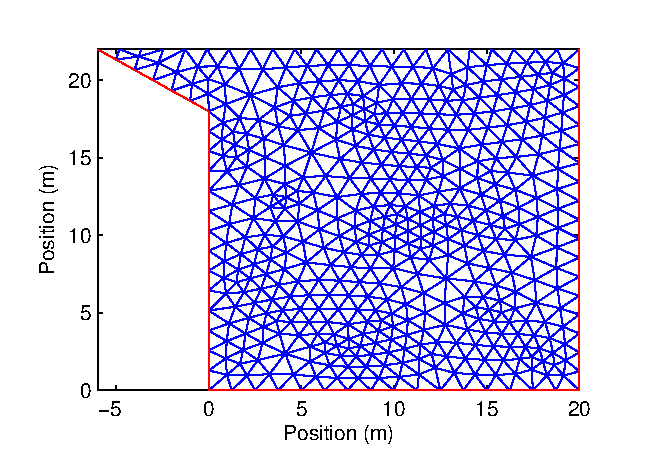
\includegraphics{images/triconvec.eps}
\caption{Definitionsmängd samt triangulering av problemuppställningen för studie av konvektion.}
\end{figure}

Svartkroppsstrålningen approximeras med första ordningens Taylorutveckling och
för varje steg löses det slutgiltiga ekvationssystemet med den
modifierade Newton-Raphson metoden. När systemet har blivit löst beräknas
medeltemperaturen på väggen. Denna används då som gissning och utvecklingspunkt
för ovan nämnda taylorutveckling. Denna process upprepas tills medeltemperaturen
ligger tillräckligt nära gissningen. Således så genomförs en rad Newtonsteg
för att hitta hur mycket som strålar från fastigheten genom svartkroppsstrålning.

Sist beräknas konvektionsparametern genom att vi vet mängden energi som transporteras
genom luften. I jämvikt gäller ekvation \eqref{eq:convectionmethod:balance}.
Här är $Q_v$ energin som flödar genom väggen, $Q_{sk}$ är energin från
svartkroppsstrålning och $Q_k$ är då energin som konvektion transporterar
för att jämvikt skall uppstå.

\begin{equation}
\label{eq:convectionmethod:balance}
Q_v + Q_{sk} = Q_k
\end{equation}

Medeltemperaturen $\bar{T}$ på väggen och referenstemperaturen $T_\infty$ är kända
vilket ger att h-värdet kan beräknas enligt

\begin{align}
Q_k &= h(\bar{T}-T_\infty) \Rightarrow \nonumber \\
h &= \frac{Q_v + Q_{sk}}{\bar{T}-T_\infty}
\end{align}
